 \documentclass[11pt,a4paper]{article}

\usepackage{pslatex}
\usepackage{inconsolata}
\usepackage[square,numbers]{natbib}
\usepackage[includehead,top=2.5cm,bottom=2.5cm,
            left=3cm,right=3cm]{geometry}
\usepackage{listings}
\usepackage{parskip}
\usepackage{amsmath}
\usepackage{amssymb}
\usepackage{bm}
\usepackage{graphicx}

\usepackage{color}
\definecolor{bluish}{rgb}{0.20,0.29,0.46}
% *always \use this last*
\usepackage[colorlinks,breaklinks,pdftex,bookmarks=true,
            linkcolor=bluish,citecolor=bluish,urlcolor=bluish]{hyperref}

\usepackage{xcolor}

\definecolor{codegreen}{rgb}{0,0.6,0}
\definecolor{codegray}{rgb}{0.5,0.5,0.5}
\definecolor{codepurple}{rgb}{0.58,0,0.82}
\definecolor{backcolour}{rgb}{0.95,0.95,0.92}

\lstdefinestyle{mystyle}{
    backgroundcolor=\color{backcolour},
    commentstyle=\color{codegreen},
    numberstyle=\tiny\color{codegray},
    stringstyle=\color{codepurple},
    basicstyle=\ttfamily\footnotesize,
    breakatwhitespace=false,
    breaklines=true,
    captionpos=b,
    keepspaces=true,
    numbers=left,
    numbersep=5pt,
    showspaces=false,
    showstringspaces=false,
    showtabs=false,
    tabsize=2
}

\lstset{style=mystyle}

\usepackage{enumitem}
\setlist{topsep=0ex,itemsep=2pt,partopsep=0pt,parsep=0pt,leftmargin=7.5mm}

% Bold face for vectors
\renewcommand{\vec}[1]{\mathbf{#1}}

% Sublist style for drafting
\renewcommand\labelenumii{\theenumii.}
\renewcommand\theenumii{\arabic{enumii}}
\renewcommand\theenumiii{\arabic{enumiii}}

\begin{document}
\lstset{language=bash}

{\huge User Guide for Spowtd v0.6.0}\\[2ex]
{\large Alex Cobb}\\[0ex]

\renewcommand{\baselinestretch}{1.18}\normalsize

This is the user guide for Spowtd, which implements the scalar
parameterization of water table dynamics described in
\citet{Cobb_et_al_2017} and \citet{Cobb_and_Harvey_2019}.

\section{The steps of scalar parameterization}
Scalar parameterization involves these essential steps:
\begin{enumerate}
\item Load water level, precipitation and evapotranspiration data;
\item Identify dry intervals and storm intervals;
\item Match intervals of rising water levels to rainstorms;
\item Construct a master rising curve;
\item Construct a master recession curve;
\item Fit a preliminary specific yield function to the master rising
  curve;
\item Jointly fit a specific yield and a conductivity (equivalently,
  transmissivity) function to the master rising and recession curves.
\end{enumerate}

\section{The spowtd script}
The \texttt{spowtd} script provides a command-line interface to
perform calculations with Spowtd.

\subsection{Dependencies}
Running the script requires Python 3 and the Python packages
\href{https://matplotlib.org/}{Matplotlib},
\href{https://numpy.org/}{Numpy}, and
\href{https://pypi.org/project/pytz/}{Pytz}.

\subsection{Using the script}
The \texttt{spowtd} script has these subcommands (typically run in
this order):
\begin{itemize}
\item \texttt{spowtd load}: Load water level, precipitation and
  evapotranspiration data.
\item \texttt{spowtd classify}: Classify data into storm and
  interstorm intervals.
\item \texttt{spowtd set-zeta-grid}: Set up water level grid for
  master curves.
\item \texttt{spowtd recession}: Assemble recession curve.
\item \texttt{spowtd rise}: Assemble rise curve.
\item \texttt{spowtd plot}: Plot data.
\item \texttt{spowtd set-curvature}: Set site curvature.
\item \texttt{spowtd simulate}: Simulate data rise curve, recession
  curve, or rising and receding intervals.
\item \texttt{spowtd pestfiles}: Generate input files for calibration
  with PEST.
\end{itemize}

The first step is to load the precipitation, evapotranspiration and
water level data.  The input text files must be in an UTF-8-compatible
encoding (ASCII is fine).  The time zone is stored with the dataset
and will be used in plots (all times are stored internally as UNIX
timestamps).  For example, to load data into a new dataset file called
\texttt{ekolongouma.sqlite3}:
\begin{lstlisting}[frame=single]
spowtd load ekolongouma.sqlite3 \
  -vvv \
  --precipitation src/precipitation_Ekolongouma.txt \
  --evapotranspiration src/evapotranspiration_Ekolongouma.txt \
  --water-level src/waterlevel_Ekolongouma.txt \
  --timezone Africa/Lagos
\end{lstlisting}
The verbosity flags (\texttt{-vvv}) are not required; they cause the
script to report more on what is being done.

Next, classify the water level and precipitation time series into
storm and interstorm intervals based on thresholds for rainfall
intensity and rates of increase in water level.  For example, this
command classifies intervals with precipitation of at least 4~mm / h
as storms, and intervals in which the water level is increasing at a
rate of least 8~mm / h as storm response.
\begin{lstlisting}[frame=single]
spowtd classify ekolongouma.sqlite3 \
  -vvv \
  --storm-rain-threshold-mm-h 4.0 \
  --rising-jump-threshold-mm-h 8.0
\end{lstlisting}
(For details on how Spowtd matches storms with rises in water level,
see Appendix~\ref{a:storm_matching}.)

At this stage the classification can be plotted.  A basic interactive
plot showing the classified water level and precipitation time series
can be produced with:
\begin{lstlisting}[frame=single]
spowtd plot time-series ekolongouma.sqlite3
\end{lstlisting}
An additional panel showing evapotranspiration is plotted if the
\texttt{-e} or \texttt{--plot-evapotranspiration} flag is passed.  The
parts of the water level time series marked as interstorms are on a
light red background, and the parts of the water level time series
marked as storm response are on a light green background.  The parts
of the precipitation time series marked as storms are on a light blue
background.  You can pan in the plot with the right mouse button and
zoom with a left mouse button, or use the magnifying glass to zoom in.
You can revert to earlier zoom and pan values with the arrow buttons.

Adding \texttt{-f} or \texttt{--flags} highlights the parts of the
water level time series that have been classified as storm response
and interstorms, and the parts of the precipitation time series
\begin{lstlisting}[frame=single]
spowtd plot time-series ekolongouma.sqlite3  -f
\end{lstlisting}
The rising intervals are highlighted in blue, intervals with rising
intervals that could not be matched to rain storms are highlighted in
magenta, and rain storms are highlighted in red.

The next step is to establish a uniform grid for water levels.  This
grid is used when storm and interstorm intervals are assembled into
rising and recession curves.
\begin{lstlisting}[frame=single]
spowtd set-zeta-grid -vvv ekolongouma.sqlite3
\end{lstlisting}

The next two steps assemble the recession and rise curves:
\begin{lstlisting}[frame=single]
spowtd recession -vvv ekolongouma.sqlite3
\end{lstlisting}

\begin{lstlisting}[frame=single]
spowtd rise -vvv ekolongouma.sqlite3
\end{lstlisting}
If desired, the correlated errors produced by imprecision in recharge
depth measurement can be taken into account when assembling the rise
curve (see Appendix~\ref{b:rise_weighting}, ``Event weighting in rise
analysis'').  To do so, pass in a relative weight to assign to these
errors, vs.\ direct errors in water level measurement, via
\texttt{--recharge-error-weight}:
\begin{lstlisting}[frame=single]
spowtd rise -vvv ekolongouma.sqlite3 --recharge-error-weight=1e3
\end{lstlisting}
To examine the error covariance matrix used in the rise curve
assembly, append the \texttt{--dump-covariance} flag and the error
covariance matrix will be written to a file (default is standard
output) as JSON.

The recession and rise curves are now assembled, and can be plotted.
\begin{lstlisting}[frame=single]
spowtd plot recession ekolongouma.sqlite3
\end{lstlisting}

\begin{lstlisting}[frame=single]
spowtd plot rise ekolongouma.sqlite3
\end{lstlisting}
These plots can be interacted with in the same way: left mouse button
to pan, right mouse button to zoom, disk icon to save.

\section{Parameterization}
Parameters are provided to \texttt{spowtd} in
\href{https://yaml.org/}{YAML} format.

Currently two types of parameter sets are supported: (1) Cubic spline
for specific yield, piecewise linear for the logarithm of
conductivity; and (2) The PEATCLSM parameterization.

The spline parameterizations look like this:
\begin{lstlisting}[frame=single]
specific_yield:
  type: spline
  zeta_knots_mm:
    - -291.7
    - -183.1
    - -15.74
    - 10.65
    - 38.78
    - 168.3
  sy_knots:  # Specific yield, dimensionless
    - 0.1358
    - 0.1671
    - 0.2541
    - 0.2907
    - 0.2892
    - 0.6857
transmissivity:
  type: spline
  zeta_knots_mm:
    - -291.7
    - -5.167
    - 168.3
    - 1000
  K_knots_km_d:  # Conductivity, km/d
    - 5.356e-3
    - 1.002
    - 6577.0
    - 8.430e+3
  minimum_transmissivity_m2_d: 7.442  # Minimum transmissivity, m2/d
\end{lstlisting}
and the PEATCLSM parameterizations look like this:
\begin{lstlisting}[frame=single]
specific_yield:
  type: peatclsm
  sd: 0.162  # standard deviation of microtopographic distribution, m
  theta_s: 0.88  # saturated moisture content, m^3/m^3
  b: 7.4  # shape parameter, dimensionless
  psi_s: -0.024  # air entry pressure, m
transmissivity:
  type: peatclsm
  Ksmacz0: 7.3  # m/s
  alpha: 3  # dimensionless
  zeta_max_cm: 5.0
\end{lstlisting}
(the text following each parameter, after the \verb|#|, is a comment
and invisible to spowtd).

The specific yield and transmissivity curves can be plotted with
\begin{lstlisting}[frame=single]
  spowtd plot WHAT parameters.yml WATER_LEVEL_MIN_CM WATER_LEVEL_MAX_CM
\end{lstlisting}
where \texttt{WHAT} is one of \texttt{specific-yield},
\texttt{conductivity} or \texttt{transmissivity},
\texttt{parameters.yml} is a YAML file containing hydraulic
parameters, and the last two arguments specify the range of water
levels over which to plot the curve.

The plotting commands \texttt{plot rise}, \texttt{plot recession} and
\texttt{plot time-series} support a parameter \texttt{-p},
\texttt{--parameters}; if a YAML file containing hydraulic parameters
is passed to one of these commands, the corresponding plot (rising
curve, recession curve, rising and receding intervals) is simulated
using those parameters.

The simulated curves and corresponding data can be obtained as text
using \texttt{spowtd simulate WHAT data.sqlite3 parameters.yml} where
\texttt{WHAT} is \texttt{rise}, \texttt{recession}, or
\texttt{intervals}.  These commands write simulated data, water level
data, and / or residuals to an output file (standard output by
default) as delimited text.  For example,
\begin{lstlisting}[frame=single]
spowtd simulate rise ekolongouma.sqlite3 parameters.yml
\end{lstlisting}
reads data from \texttt{ekolongouma.sqlite3} and parameters from the
file \texttt{parameters.yml} and writes the assembled and simulated
rise curves to standard output.  The curves are simulated over the
range of water levels in the data, so plots from different SQLite
files may look different even if the parameters are identical.

To simulate (or plot) recession requires setting the large-scale
curvature of the site.  The command
\begin{lstlisting}[frame=single]
  spowtd set-curvature ekolongouma.sqlite3 1.0
\end{lstlisting}
sets the site curvature to $1~\text{m}/\text{km}/\text{km}$, whereafter
\begin{lstlisting}[frame=single]
  spowtd simulate recession ekolongouma.sqlite3 parameters.yml
\end{lstlisting}
simulates the water table recession.

\section{Calibration with PEST}
The simulation scripts make it possible to calibrate the specific
yield and transmissivity functions against rise and recession of the
water level using the \href{https://pesthomepage.org/}{PEST} software
package and tools for model-independent parameter estimation and
uncertainty analysis.  It should also be possible to calibrate using
\href{https://www.usgs.gov/software/pest-software-suite-parameter-estimation-uncertainty-analysis-management-optimization-and}{PEST++},
which is designed to have the same text-based interface, by following
a similar procedure.

PEST is a highly configurable set of tools.  One of its strengths is
that it is possible to start with a fairly simple approach and
incorporate more sophisticated functionality as it is needed.  As an
introduction, we illustrate calibration of specific yield parameters
against the rise curve.

For a calibration with PEST, you need to create five text files:
\begin{enumerate}
\item A PEST control file (\texttt{.pst}), which configures how PEST
  will perform the calibration (including identifying the other files
  used during calibration);
\item A parameter template file (\texttt{.tpl}), into which PEST will
  substitute parameter values in a format that can be read by Spowtd;
\item An output template file, or PEST ``instruction file''
  (\texttt{.ins}), which teaches PEST how to extract ``observations''
  from \texttt{spowtd simulate} output;
\item A vector of initial parameters (\texttt{.par}) to start the
  calibration; and
\item A script to execute the rise simulation.
\end{enumerate}

The first step is to create the PEST control file (\texttt{.pst})
following the PEST documentation \citep{Doherty_2010}.  For a PEATCLSM
parameterization, the control file will describe the four PEATCLSM
parameters for specific yield (\texttt{sd}, \texttt{theta\_s},
\texttt{b}, and \texttt{psi\_s}), each with their own parameter group.
The control file must also include an ``observation data'' section
with a single line giving mean dynamic storage for each water level in
the rise curve. The ``model command line'' section must provide the
command line needed to run the script to generate the rise curve.  The
script itself can be, for example, a bash script that calls
\texttt{spowtd simulate rise}.  Finally, the ``model input/output''
section specifies the path to the parameter template file, the path to
the the parameter file that PEST will create by substituting parameter
values into the template, the path to the instruction file
(\texttt{.ins}) that PEST uses to interpret the simulation output, and
the path to the output file created by a single run of the simulation
script.

The parameter template file (\texttt{.tpl}) and the parameter vector
file (\texttt{.par}) are created by replacing values in a Spowtd YAML
parameter file by placeholders, as described in the PEST
documentation.  In the case of calibration of PEATCLSM specific yield
parameters against a rise curve, the template file might look like this:
\begin{lstlisting}[frame=single]
ptf @
specific_yield:
  type: peatclsm
  sd: @sd                      @
  theta_s: @theta_s                 @
  b: @b                       @
  psi_s: @psi_s                   @
transmissivity:
  type: peatclsm
  Ksmacz0: 7.3  # m/s
  alpha: 3  # dimensionless
  zeta_max_cm: 5.0
\end{lstlisting}
and an initial parameter vector file might look like this:
\begin{lstlisting}[frame=single]
double point
          sd    0.162                      1.000000         0.000000
     theta_s    0.88                       1.000000         0.000000
           b    7.4                        1.000000         0.000000
       psi_s    -0.024                     1.000000         0.000000
\end{lstlisting}
In this example, the parameters \texttt{Ksmacz0} and \texttt{alpha}
are not included in the parameter vector file because only the rise
curve is being fitted.  The parameters of the transmissivity are not
free (they do not affect the rising curve fit), and therefore these
values are fixed in the template file and omitted from the parameter
vector file.

To verify the format of a template \texttt{rise\_pars.yml.tpl} and
initial parameters \texttt{rise\_init.par}, use the PEST
\texttt{tempchek} command:
\begin{lstlisting}[frame=single]
tempchek rise_pars.yml.tpl rise_pars.yml rise_init.par
\end{lstlisting}
This command should exit without errors and produce a valid parameter
file at \texttt{rise\_pars.yml}.

The parameter file can then be verified by running your script.  Your
script might, for example, contain the command
\begin{lstlisting}[frame=single]
spowtd simulate rise ekolongouma.sqlite3 rise_pars.yml -o rise_observations.yml --observations
\end{lstlisting}
which generates simulated dynamic storage values (without water levels
or measured dynamic storage values) in
\texttt{rise\_observations.yml}; in PEST, simulated output values are
referred to as ``observations.''

The resulting output file can then be checked against a PEST
instruction file (\texttt{.ins}) that you create for extracting
observation data, which might be called
\texttt{rise\_observations.ins}, using the PEST command
\texttt{inschek}:
\begin{lstlisting}[frame=single]
inschek rise_observations.ins rise_observations.yml
\end{lstlisting}

To then ensure that the correct initial parameters are used in the
calibration, substitute these into the control file using
\texttt{parrep}
\begin{lstlisting}[frame=single]
parrep rise_init.par rise_calibration.in.pst rise_calibration.pst
\end{lstlisting}

To then calibrate specific yield parameters against the rise curve
(alone) using the PEST control file \texttt{rise\_calibration}, call:
\begin{lstlisting}[frame=single]
pestchek rise_calibration &&
(pest rise_calibration.pst ;
 tempchek rise_pars.yml.tpl rise_opt.yml rise_calibration.par)
\end{lstlisting}
These commands check the PEST control file, perform the calibration,
and then substitute the calibrated parameter values from
\texttt{rise\_calibration.par} into \texttt{rise\_opt.yml}.

You can then examine the fit by plotting the rise curve with the
calibrated parameters:
\begin{lstlisting}[frame=single]
spowtd plot rise ekolongouma.sqlite3 --parameters rise_opt.yml
\end{lstlisting}

\subsection{Generating PEST input files with Spowtd}
As a convenience, Spowtd can generate input files for calibration with
PEST, either against the rise curve (\texttt{spowtd pestfiles rise})
or against both rise and recession curves (\texttt{spowtd pestfiles
  curves}).  The arguments to both subcommands are the same.  Taking
calibration against the rise curve as an example, a template file
can be created with
\begin{lstlisting}[frame=single]
spowtd pestfiles rise ekolongouma.sqlite3 parameters.yml tpl \\
  -o rise_parameters.yml.tpl
\end{lstlisting}
An instruction file can similarly be created with
\begin{lstlisting}[frame=single]
spowtd pestfiles rise ekolongouma.sqlite3 parameters.yml ins \\
  -o ekolongouma_rise_observations.ins
\end{lstlisting}
and a control file can be created with
\begin{lstlisting}[frame=single]
spowtd pestfiles rise ekolongouma.sqlite3 parameters.yml pst \\
  -o ekolongouma_rise_calibration.in.pst
\end{lstlisting}
The template and instruction files can be used as-is.  The generated
PEST control file will require substitution of valid starting
parameters and bounds, substitution of paths to input files and the
invocation for simualtion, adjustment of PEST control parameters, etc.

\bibliographystyle{unsrtnat}
\bibliography{user_guide.bib}

\appendix

\section{Matching of storms and water table rise}
\label{a:storm_matching}

For construction of rise curves, Spowtd matches intervals of rapidly
increasing water level (``rises'') to intervals of heavy rain
(``storms'') in such a way that each storm is matched to no more than
one rise and each rise is matched to no more than one storm.  This
matching is performed in two steps.  First, all storms and rises that
overlap in time are matched.  This first step may result in matching
from a single storm to multiple rises and vice versa.  This step is
followed by an arbitration step based on a variant of the Gale-Shapley
deferred acceptance algorithm for the stable matching problem: it
finds a set of matches between storms and rises that is stable in the
sense that, by switching a pair of matches between storms and rises,
one cannot improve the agreement in duration and start time for both
matches.

The arbitration step favors agreement in duration over agreement in
start time in matches by using a property of the Gale-Shapley
algorithm: it is guaranteed to yield the stable matching that is most
favorable for the proposing parties, and least favorable for the
parties accepting or rejecting proposals.  In matching between storms
and rises, each storm tries to match with the rise with the closest
duration; the rise is then able to reject that first match if another
storm with a closer start time proposes a match.  However, a storm
that is already matched with a rise with a more similar duration will
never propose to the rise with a closer start time.  Thus, arbitration
results in the stable matching that results in the best agreement in
duration between storms and rises.

Note that matching may still result in bad mismatches in storm and
rise duration depending on the thresholds set for identifying intense
rain (for storms) and rapid increase in water level (for rises).  If
differences between storm and rise duration are larger than you think
they should be, try adjusting one of these thresholds to get better
agreement.

\section{Event weighting in rise analysis}
\label{b:rise_weighting}

Assembly of recession curves benefits from the fact that both water
level and time usually can be measured fairly accurately.  In
contrast, rise events may be affected by large errors in measurement
of the recharge depth, either because of the difficulties in measuring
the precipitation that passes through the canopy and litter to reach
the water table, or because of spatial separation or scale differences
between where precipitation is measured and where the water table
response is evaluated.

In some cases the error in recharge depth measurement may be large
enough to cause problems in assembling a reasonable rise curve.
Because each rise event is represented as a straight line segment
between the water level and dynamic storage at the beginning and end
of the event, an error in the recharge depth is manifested as an error
in slope of this segment.  In the case of a range of water levels
where specific yield is approximately uniform so that the true slope
of the rise curve is approximately constant, this error in slope
causes an error in observed cumulative recharge that increases in
proportion to distance from the center of the rise event line segment
(Fig.~\ref{fig:rise_event_error}).  A single event spans multiple
water levels, and thus affects multiple equations.  To reduce the
impact of a single event that spans a large number of water levels and
happens to have a large error in recharge depth on the rise curve,
Spowtd will provide a scheme to ensure that events are effectively
weighted equally, and which explicitly considers the effects of a bad
estimate of recharge depth on observations of the rise event at
multiple water levels.

\begin{figure}[b!]
  \centerline{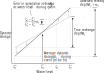
\includegraphics[scale=1]{build/doc/rise_event_error.pdf}}
  \caption{Model for error in recharge depth observations.}
  \label{fig:rise_event_error}
\end{figure}

As discussed in \citet{Cobb_et_al_2017} and
\citet{Cobb_and_Harvey_2019}, the assembly of the rise curve involves
finding the mean dynamic storage $S_j$ during each rise event $j$
(Fig.~\ref{fig:rise_event_error}), and results in the following
equation:
\begin{equation}
  R_{ij} + S_j = \frac{1}{|J_i|}\left(\sum_{j'\in J_i} R_{ij'} + S_{j'}\right)
\end{equation}
where $J_i$ is the set of rises crossing $\zeta_i$, $|J_i|$ is the
size (cardinality) of $J_i$ and $j'$ is a dummy index of summation.
Note that $j$ indexes rise events, while $i$ indexes water levels
$\zeta_i$ (Table~\ref{tab:rise_notation}).

Rearranging, for each of the $|J_i|$ rise events $j$ that cross a
discrete water level $i$, we have an equation
\begin{equation}
  \left(\frac{1}{|J_i|}\sum_{j' \in J_i} S_j' \right) - S_j = R_{ij} - \frac{1}{|J_i|} \sum_{j' \in J_i} R_{ij'}
\end{equation}
which can be written in matrix form with typical row
\begin{equation}
  \label{eq:rise_vector_equation}
  \left[
    \begin{array}{cccccc}
      \frac{1}{J_i} & \frac{1}{J_i} & \ldots & \frac{1}{J_i} - 1 & \ldots & \frac{1}{J_i}
    \end{array}
\right]\left[
  \begin{array}{c}
    S_1 \\
    S_2 \\
    \vdots \\
    S_j \\
    \vdots \\
    S_{J-1}
  \end{array}
\right]
 = \left[R_{ij} - \frac{1}{|J_i|}\sum_{j' \in J_i} R_{ij'}\right].
\end{equation}
This represents $|J_i|$ equations. The quantity on the right is a
scalar; there is one such equation---with the same row and column
vectors on the left, but a different row vector on the right---for
each rise event $j$ of the $|J_i|$ rise events crossing water level
$i$.  The mean dynamic storage $S_J$ for rise event $J$ is set to 0
and excluded from the unknowns to make the problem nonsingular; after
solving for the other dynamic storage values, a constant is subtracted
from all of these to define the dynamic storage as zero when the water
level is at the peat surface ($\zeta = 0$), as described in
\citet{Cobb_and_Harvey_2019}.

\begin{table}[b!]
  \centering
  \begin{tabular}{cp{10.8cm}}
    \emph{Symbol} & \emph{Definition} \\
    \hline
    $\langle\cdot\rangle$ & Expected value \\
    $e_{ij}$ & Error in cumulative recharge at water level $i$ during event $j$ \\
    $f_{ij}$ & Weighting coefficient for error in cumulative recharge
               at water level $i$ for event $j$\\
    $i$ & Index over discrete water levels $\zeta_i$\\
    $j$ & Index over rise events\\
    $J_i$ & Set of rise events crossing water level $i$\\
    $k$ & Index over equations; enumerates $(i, j)$ pairs identifying water levels crossed by recharge events \\
    $R_{ij}$ & True cumulative recharge at water level $i$ during event $j$ \\
    $\widehat{R}_{ij}$ & Observed cumulative recharge at water level $i$ during event $j$ \\
    $R_j$ & True total recharge depth during rise event $j$ \\
    $S$ & Dynamic storage \\
    $S_j$ & Average dynamic storage during event $j$ \\
    $S_y$ & Specific yield \\
    $\alpha_j$ & Error in recharge depth during rise event $j$ \\
    $\epsilon_k$ & Error in equation $k$ \\
    $\zeta$ & Water level \\
  \end{tabular}
  \caption{Notation for assembly of rise curves}
  \label{tab:rise_notation}
\end{table}

The set of equations (\ref{eq:rise_vector_equation}) for the average
dynamic storage $S_j$ during each event can be written as a matrix
equation
\begin{equation}
  \vec{A}\vec{x} = \vec{b}
\end{equation}
where $\vec{A}$ is a dense matrix with $K = \sum_i |J_i|$ rows and $J - 1$
columns, $\vec{x}$ is the vector of unknown dynamic storage values $S$
and $\vec{b}$ contains the right-hand-side values from
equation~\ref{eq:rise_vector_equation}.

Ideally, the true recharge depth $R_j$ for a storm $j$ would be known,
and this system of equations $\vec{A}\vec{x} = \vec{b}$ would have a
solution after elimination of redundant equations.  In practice,
errors in recharge depth affect all equations and introduce covariance
among the components of the error vector $\bm{\epsilon}$ associated
with the system of equations $\vec{A}\vec{x} = \vec{b}$.

Suppose recharge depth observations $\widehat{\mathbf{R}}$ are
affected by multiplicative independent errors $\bm{\alpha}$, each
identically distributed with mean 1 and variance $\text{var}(\alpha)$.
For a rise event $j$, our observations at every water level $i$
crossed by the rise event are contaminated by that error $\alpha_j$:
\begin{equation}
  \widehat{R}_{ij} = f_{ij}\alpha_j R_{ij}
\end{equation}
with $f_{ij}$ defined as
\begin{equation}
f_{ij} = \frac{\zeta_i - \overline{\zeta_j}}{\zeta_j^* - \zeta^o_j}
\end{equation}
where $\zeta^o_j$ is the water level at the beginning and $\zeta^*_j$
the water level at the end of event $j$
(Fig.~\ref{fig:rise_event_error}).

The error $e_{ij}$ in each observed recharge depth is
\begin{equation}
  \label{eq:recharge_error_mean}
  e_{ij} = \widehat{R}_{ij} - R_{ij} = (\alpha_j - 1) R_j f_{ij}
\end{equation}
with zero mean
\begin{equation}
  \langle e_{ij} \rangle = \left[\langle \alpha_j\rangle - 1\right] R_j f_{ij} = 0.
\end{equation}

The error $\epsilon_k$ in the $k^\text{th}$ equation is a linear
combination of the errors $e_{ij}$ in the recharge depth
\begin{equation}
  \label{eq:epsilon_k}
  \epsilon_k = e_{ij} - \beta_i
\end{equation}
where $i$ and $j$ are the water level $i$ and rise $j$ associated with
the $k$th equation, and $\beta_i$ is the average error across storm
events crossing water level $i$
\begin{equation}
  \label{eq:beta_i}
  \beta_i = \frac{1}{|J_i|}\sum_{j' \in J_i} e_{ij'}
\end{equation}

We hypothesize that we can obtain a truer fit by deriving an estimate
of the variance-covariance matrix $\bm{\Omega}$ of the error vector,
and then solving the generalized least-squares problem
\begin{equation}
  \label{eq:generalized_lsq}
  \vec{A}^T \bm{\Omega}^{-1} \vec{A} \vec{x} = \vec{A}^T \bm{\Omega}^{-1} \vec{b}.
\end{equation}

We will use our model for the recharge depth error $\alpha$ to derive
an estimate for the covariance between elements of the error vector
$\bm{\epsilon}$ (variance of error vector $\bm{\epsilon}$).

The covariance $\text{cov}(\epsilon_{k_1}, \epsilon_{k_2})$
between two components of the error vector is the expected value of
the product of their deviations.  Because the errors $\vec{e}$ in
recharge have zero mean (\ref{eq:recharge_error_mean}), inspection of
(\ref{eq:epsilon_k}) shows that the elements of $\bm{\epsilon}$ also
have zero mean, and therefore an element of the variance-covariance
matrix of the error vector $\bm\epsilon$ is given by
\begin{equation}
  \label{eq:epsilon_covariance}
  \text{cov}\left(\epsilon_{k_1}, \epsilon_{k_2}\right) = \langle \epsilon_{k_1} \epsilon_{k_2}\rangle
\end{equation}
which, after substitution from (\ref{eq:epsilon_k}), expands to
\begin{equation}
  \label{eq:epsilon_covariance_terms}
  \text{cov}\left(\epsilon_{k_1}, \epsilon_{k_2}\right) = \left\langle e_{i_1 j_1} e_{i_2 j_2}\rangle - \langle e_{i_1 j_1}\beta_{i_2}\rangle - \langle e_{i_2 j_2}\beta_{i_1}\rangle + \langle \beta_{i_1}\beta_{i_2} \right\rangle
\end{equation}

We first derive expressions for the terms in this equation
(\ref{eq:epsilon_covariance_terms}).  It is convenient to divide these
terms by the variance $\text{var}(\alpha)$ in $\alpha$.  The expected
product of pairs of errors $e_{ij}$ in observed recharge depth is
\begin{equation}
  \left\langle e_{i_1, j_1}\, e_{i_2, j_2}\right\rangle = \left[ \langle\alpha_{j_1} \alpha_{j_2}\rangle - 1 \right] R_{j_1} R_{j_2} f_{i_1 j_1} f_{i_2 j_2}.
\end{equation}
Because the components of the error $\bm{\alpha}$ are independent, the
expected value of their product
$\langle\alpha_{j_1} \alpha_{j_2}\rangle$ is $1 + \text{var}(\alpha)$
if $j_1 = j_2$ and 1 otherwise.  Therefore, the expected product of
recharge depth observation errors, normalized by $\text{var}(\alpha)$,
is
\begin{equation}
  \label{eq:e_covariance}
  \frac{\left\langle e_{i_1, j_1}\, e_{i_2, j_2}\right\rangle}
       {\text{var}(\alpha)} =
    R_{j_1}^2 f_{i_1 j_1} f_{i_2 j_1}\, [j_1 = j_2].
\end{equation}
where we use the Iverson bracket $[P\,]$ to denote the indicator
function that takes the value 1 if the statement $P$ within the
brackets is true and 0 otherwise.

The terms $\langle e_{i_1 j_1}\, \beta_{i_2}\rangle$, again normalized
by the variance $\text{var}(\alpha)$ of $\alpha$, after substitution
and rearrangement, are given by
\begin{equation}
  \frac{\langle e_{i_1 j_1}\, \beta_{i_2}\rangle}{\text{var}(\alpha)} = \frac{1}{|J_{i_2}|}\sum_{j' \in J_{i_2}} f_{i_2 j'} \frac{\langle e_{i_1 j_1} e_{i_2 j'} \rangle}{\text{var}(\alpha)}
\end{equation}
which, because any $j$ appears at most once in $J_{i_2}$, can be
expressed, again using the Iverson bracket, as
\begin{equation}
  \label{eq:e_beta_covariance}
  \frac{\langle e_{i_1 j_1}\, \beta_{i_2}\rangle}{\text{var}(\alpha)} = \frac{R_{j_1}^2 f_{i_1 j_1} f_{i_2 j_1}}{|J_{i_2}|} [j_1 \in J_{i_2}]
\end{equation}

Finally, the terms $\langle\beta_{i_1}\,\beta_{i_2}\rangle$ are given by
substitution from (\ref{eq:beta_i}) as
\begin{equation}
  \langle\beta_{i_1}\,\beta_{i_2}\rangle =
  \left\langle
  \left(\frac{1}{|J_{i_1}|}\sum_{j' \in J_{i_1}} e_{i_1 j'}\right)
  \left(\frac{1}{|J_{i_2}|}\sum_{j' \in J_{i_2}} e_{i_2 j'}\right)
  \right\rangle
\end{equation}
which, after normalizing by the variance of $\alpha$, expands to
\begin{equation}
  \frac{\langle\beta_{i_1}\,\beta_{i_2}\rangle}{\text{var}(\alpha)} =
  \frac{1}{|J_{i_1}| |J_{i_2}|}
    \sum_{j' \in J_{i_1}, j'' \in J_{i_2}} \frac{\left\langle e_{i_1 j'}\, e_{i_2 j''} \right\rangle}{\text{var}(\alpha)}
\end{equation}
and then, using (\ref{eq:e_covariance}), simplifies to
\begin{equation}
  \label{eq:beta_covariance}
  \frac{\langle\beta_{i_1}\,\beta_{i_2}\rangle}{\text{var}(\alpha)} =
  \frac{1}{|J_{i_1}| |J_{i_2}|} \sum_{j' \in J_{i_1}\cap J_{i_2}} R_{j'}^2 f_{i_1 j'} f_{i_2 j'}
\end{equation}

Finally, substituting from the expressions (\ref{eq:e_covariance}),
(\ref{eq:e_beta_covariance}) and (\ref{eq:beta_covariance}) for terms
in (\ref{eq:epsilon_covariance_terms}), we have the elements
$\text{cov}\left(\epsilon_{k_1}, \epsilon_{k_2} \right)$ of the
variance-covariance matrix $\bm{\Omega}$ of the error vector
$\mathbf{\epsilon}$, normalized by the recharge depth error variance
$\text{var}(\alpha)$, as
\begin{align}
\begin{split}
\label{eq:epsilon_normalized_covariance}
  \frac{\text{cov}\left(\epsilon_{k_1}, \epsilon_{k_2}\right)}{\text{var}(\alpha)} =
  &R_{j_1}^2 f_{i_1 j_1} f_{i_2 j_1}\, [j_1 = j_2] \\
  &- \frac{R_{j_1}^2 f_{i_1 j_1} f_{i_2 j_1}}{|J_{i_2}|} [j_1 \in J_{i_2}]\\
  &- \frac{R_{j_2}^2 f_{i_2 j_2} f_{i_1 j_2}}{|J_{i_1}|} [j_2 \in J_{i_1}]\\
  &+ \frac{1}{|J_{i_1}| |J_{i_2}|} \sum_{j' \in J_{i_1}\cap J_{i_2}} R_{j'}^2 f_{i_1 j'} f_{i_2 j'}
\end{split}
\end{align}
We do not have the true recharge depths $R_j$, but only recharge depth
observations $\widehat{R}_j$, so we approximate the covariance terms
using these observations instead.  We note in passing that the
expected value of $\widehat{R}_j^2$ is
$[1 + \text{var}(\alpha)]R_j^2$, but because all terms are scaled by
the same scalar $1 + \text{var}(\alpha)$, neglecting this does not
change the equations analytically.

For numerical reasons, to keep the
norm of $\bm{\Omega}$ close to 1, we nondimensionalize the recharge
observations $\widehat{R}_j$ by dividing them by their mean prior to
further calculations (dividing $\bm{\Omega}$ by a scalar has no
analytical effect because its inverse appears once on the left and the
right of (\ref{eq:generalized_lsq})).

Using (\ref{eq:epsilon_normalized_covariance}), we populate the
variance-covariance matrix
$\bm{\Omega} = \text{var}(\mathbb\epsilon)$, compute its inverse, and
then solve the generalized least-squares problem
(\ref{eq:generalized_lsq}) to obtain the average storage
$S_j, j \in \{1, 2, \ldots, J - 1\}$ to a constant from the entries in
$\vec{x}$.

\end{document}
